\begin{center}
\justifying
\chapter{Work Done}

This work addresses three complementary security problems spanning system monitoring and cryptographic analysis. First, it proposes a role-aware representation learning framework for log-based anomaly detection that addresses the structural limitations of existing parsing-free methods. The framework operates directly on raw log text without any dependency on log parsers, while explicitly modeling the functional roles of tokens to produce richer and more interpretable log representations. Second, it investigates the vulnerability of XOR-based secret image sharing schemes under learning-based attacks by employing autoencoder architectures to reconstruct images from incomplete share sets. Third, it performs a cryptanalysis of a chaos-based medical image encryption scheme, demonstrating that structural weaknesses such as plaintext-independent keystream generation and separable permutation-diffusion design enable complete decryption under a chosen-plaintext attack.


% ===========================
% PROBLEM 1
% ===========================

\section{Work Done for Problem 1: Role-Aware Log Anomaly Detection}

\subsection{Enhanced Preprocessing}

Unlike NeuralLog~\cite{neurallog2021}, which discards all numeric tokens prior to 
encoding, our preprocessing pipeline retains numeric tokens as first-class vocabulary 
items. Log messages are normalized to lowercase and tokenized using common delimiters 
such as whitespace, colons, and commas. Numeric tokens such as HTTP status codes, 
memory values, retry counts, and block identifiers are preserved, as they frequently 
carry anomaly-relevant signal that uniform removal would destroy.

\begin{figure}[H]
\centering
\vspace{-0.5em}
\begin{tikzpicture}[
    node distance=0.5cm,
    startstop/.style={rectangle, rounded corners, minimum width=2cm, minimum height=0.5cm, text centered, draw=black, fill=white!10, font=\scriptsize},
    process/.style={rectangle, minimum width=2.5cm, minimum height=0.5cm, text centered, draw=black, fill=white!5, font=\scriptsize},
    model/.style={rectangle, minimum width=2.5cm, minimum height=0.5cm, text centered, draw=black, fill=white!5, font=\scriptsize},
    arrow/.style={->, >=Stealth}
]
\node (in1) [startstop] {Raw Logs};
\node (pro1) [process, below=of in1] {Tokenization \& BERT};
\node (pro2) [process, below=of pro1] {Role Induction};
\node (pro3) [process, below=of pro2] {Role-Aware Pooling};
\node (mod1) [model, below=of pro3] {Transformer};
\node (out1) [startstop, below=of mod1] {Classification};
\draw [arrow] (in1) -- (pro1);
\draw [arrow] (pro1) -- (pro2);
\draw [arrow] (pro2) -- (pro3);
\draw [arrow] (pro3) -- (mod1);
\draw [arrow] (mod1) -- (out1);
\end{tikzpicture}
\vspace{-0.5em}
\caption{Log Anomaly Detection Pipeline}
\label{fig:architecture}
\end{figure}

\subsection{Token Encoding with BERT}

Each preprocessed log message is tokenized using WordPiece tokenization~\cite{schuster2012japanese}, which decomposes rare or domain-specific terms into frequent subword units, eliminating out-of-vocabulary issues common in technical log vocabularies. Token embeddings are generated using BERT-base (12 layers, 768 hidden dimensions)~\cite{devlin2018bert}, producing a set of contextual representations $\mathbf{H} = [\mathbf{h}_1, \mathbf{h}_2, \ldots, \mathbf{h}_n]$ where each $\mathbf{h}_i \in \mathbb{R}^{768}$ encodes a token in the context of its surrounding message.

\subsection{Latent Token Role Induction}

The central contribution of this work is the latent token role induction mechanism. We postulate that tokens in log messages fulfill distinct functional roles — some denote system states, others identify components, others describe operations, and some convey quantitative or spatial information — and that modeling these roles explicitly produces representations better suited to anomaly detection than uniform averaging.

\subsubsection{Role Categories}

Five latent role categories are defined: \textit{state} (e.g., error, timeout, success), \textit{entity} (e.g., node, disk, process), \textit{action} (e.g., detected, killed, restarted), \textit{quantity} (e.g., error codes, counts, identifiers), and \textit{location} (e.g., file paths, registers, directories). Critically, no manual annotation of these roles is required; they are discovered automatically through end-to-end training on sequence-level anomaly labels.

\subsubsection{Role Induction Network}

For each token $t_i$ with BERT embedding $\mathbf{h}_i \in \mathbb{R}^{768}$, a two-layer feedforward network predicts a soft role distribution: \[ \mathbf{r}_i = \text{softmax}(W_r \cdot \text{ReLU}(W_h \mathbf{h}_i + b_h) + b_r) \] where $W_h \in \mathbb{R}^{256 \times 768}$ and $W_r \in \mathbb{R}^{5 \times 256}$ are learned weight matrices and $\mathbf{r}_i \in \mathbb{R}^5$ is the resulting probability distribution over the five role categories. A role-aware token representation is then formed by modulating the BERT embedding with role information: \[ \mathbf{t}_i = \mathbf{h}_i \odot \mathbf{W}_e \mathbf{r}_i \] where $\mathbf{W}_e \in \mathbb{R}^{768 \times 5}$ is a learned role embedding matrix and $\odot$ denotes element-wise multiplication. Since the role induction network is trained solely from the anomaly detection gradient signal, tokens that contribute similarly to detection automatically receive similar role assignments.

\subsection{Role-Aware Message Representation}

Rather than uniformly averaging all token embeddings as in NeuralLog, we construct a structured message representation by performing separate pooling operations for each role category: \[ \mathbf{m} = [\mathbf{m}_{\text{state}};\, \mathbf{m}_{\text{entity}};\, \mathbf{m}_{\text{action}};\, \mathbf{m}_{\text{quantity}};\, \mathbf{m}_{\text{location}}] \] where each role-specific pool is computed as a soft weighted average: \[ \mathbf{m}_k = \frac{\sum_{i=1}^{n} r_{i,k} \cdot \mathbf{t}_i} {\sum_{i=1}^{n} r_{i,k}} \] and $r_{i,k}$ is the probability that token $i$ belongs to role $k$. The resulting message vector $\mathbf{m} \in \mathbb{R}^{3840}$ concatenates five role-specific sub-vectors of 768 dimensions each, preserving structural distinctions that a single averaged vector would collapse.

\subsection{Sequence Modeling}

Log sequences are constructed using a sliding window of size 20 and step 1, following the protocol of NeuralLog~\cite{neurallog2021}. Sinusoidal positional encodings~\cite{vaswani2017attention} are added to each message representation to inject ordering information: \[ \mathbf{x}_i = \mathbf{m}_i + \mathbf{p}_i \] A single-layer Transformer encoder with 12 attention heads and a feedforward dimension of 2048 is then applied over the sequence to model temporal dependencies among log messages: \[ \mathbf{X}' = \text{TransformerEncoder}(\mathbf{X}) \]

\subsection{Classification and Training}

A max-pooling operation is applied over the sequence output to obtain a fixed-size representation, which is passed through a fully connected layer followed by softmax to produce the anomaly prediction: \[ P(\text{anomaly} \mid \mathbf{s}) = \text{softmax}(W_c \mathbf{s} + b_c) \] The full framework is trained end-to-end using binary cross-entropy loss: \[ \mathcal{L} = -\sum_{j} y_j \log \hat{y}_j + (1 - y_j)\log(1 - \hat{y}_j) \] with the AdamW optimizer at a learning rate of $3 \times 10^{-4}$, a batch size of 64, and a dropout rate of 0.1. Early stopping is applied after 5 epochs without improvement, with a maximum of 20 training epochs. Sequence-level anomaly labels are the only supervision required; token roles emerge entirely through backpropagation.
% ===========================
% PROBLEM 2
% ===========================

\section{Problem 2: Attack on XOR-Based Secure Image Sharing using Autoencoders}

A $(4,4)$ plain random XOR secret sharing scheme was used for all experiments.

For each secret image:
\begin{itemize}
    \item Three shares are generated randomly using independent Bernoulli sampling,
    \item The fourth share is computed as the XOR of the binarized secret image with the first three random shares.
\end{itemize}

Formally, let $S$ denote the binarized secret image and $R_1, R_2, R_3$ denote independent random shares. The fourth share $R_4$ is computed as: \[ R_4 = S \oplus R_1 \oplus R_2 \oplus R_3. \]

This guarantees that: \[ S = R_1 \oplus R_2 \oplus R_3 \oplus R_4. \]

Under classical cryptographic assumptions, any strict subset of fewer than four shares is information-theoretically insufficient to deterministically recover the secret. All shares are generated dynamically during training to prevent memorization and ensure statistical variability across epochs.

\begin{figure}[H]
\centering
\vspace{-0.5em}
\begin{tikzpicture}[
    node distance=0.5cm,
    startstop/.style={rectangle, rounded corners, minimum width=3cm, minimum height=0.5cm, text centered, draw=black, fill=white!10, font=\scriptsize},
    process/.style={rectangle, minimum width=3cm, minimum height=0.5cm, text centered, draw=black, fill=white!5, font=\scriptsize},
    model/.style={rectangle, minimum width=3cm, minimum height=0.5cm, text centered, draw=black, fill=white!5, font=\scriptsize},
    arrow/.style={->, >=Stealth}
]

% Nodes
\node (in1) [startstop] {Secret Image $S$ (MNIST)};
\node (pro1) [process, below=of in1] {Binarization \& Resize ($128 \times 128$)};
\node (pro2) [process, below=of pro1] {XOR Share Generation ($R_1, R_2, R_3, R_4$)};
\node (pro3) [process, below=of pro2] {Share Concatenation (Channel Dimension)};
\node (mod1) [model, below=of pro3] {Residual CNN Decoder ($f_\theta$ or $g_\phi$)};
\node (pro4) [process, below=of mod1] {Sigmoid Output Layer};
\node (out1) [startstop, below=of pro4] {Reconstructed Image $\hat{S}$};
\node (eval) [startstop, below=of out1] {Evaluation: SSIM \& PSNR};

% Arrows
\draw [arrow] (in1) -- (pro1);
\draw [arrow] (pro1) -- (pro2);
\draw [arrow] (pro2) -- (pro3);
\draw [arrow] (pro3) -- (mod1);
\draw [arrow] (mod1) -- (pro4);
\draw [arrow] (pro4) -- (out1);
\draw [arrow] (out1) -- (eval);

\end{tikzpicture}
\vspace{-0.5em}
\caption{Learning-Based Attack Pipeline on XOR Secret Sharing Scheme}
\label{fig:xor_attack_pipeline}
\end{figure}

\subsection{Dataset Preparation}

The MNIST dataset was used for training and evaluation. All images were:
\begin{itemize}
    \item Normalized to the range $[0,1]$,
    \item Resized to a spatial resolution of $128 \times 128$,
    \item Treated as single-channel grayscale inputs.
\end{itemize}

Share generation was performed on-the-fly during training to prevent fixed share–image pair memorization and to improve generalization of the learning-based decoder.

\subsection{Learning-Based Reconstruction Framework}

To evaluate the vulnerability of XOR-based secret sharing under learning-based
attacks, two distinct decoder configurations were investigated.

\subsubsection{Configuration 1: Decoder Trained on All Four Shares}

In the first configuration, the neural decoder is trained using all four shares as input.

\paragraph{Input Representation}
The four generated shares are concatenated along the channel dimension to form a 4-channel tensor of size $128 \times 128 \times 4$.

\paragraph{Training Objective}
The decoder learns a mapping: \[ f_\theta : \mathbb{R}^{128 \times 128 \times 4} \rightarrow \mathbb{R}^{128 \times 128}, \] where the target output is the original secret image. Binary cross-entropy loss is used for optimization, and the model is trained for 20 epochs using the Adam optimizer.

\paragraph{Evaluation Scenarios}
The trained model is evaluated under multiple share availability conditions:
\begin{itemize}
    \item All four shares available,
    \item One share missing (replaced with a zero/blank share),
    \item Two shares missing (replaced with zero shares),
    \item Three shares missing (only one share available).
\end{itemize}

This configuration models an attacker who has full exposure during training but encounters incomplete share availability during inference.

\subsubsection{Configuration 2: Decoder Trained on Three Consecutive Shares}

In the second configuration, the decoder is trained using only three consecutive shares without wrap-around. The valid combinations considered are:
\begin{itemize}
    \item Shares $\{1,2,3\}$,
    \item Shares $\{2,3,4\}$.
\end{itemize}

\paragraph{Input Representation}
The selected three shares are concatenated to form a 3-channel tensor of size
$128 \times 128 \times 3$.

\paragraph{Training Objective}
The decoder learns the mapping:
\[ g_\phi : \mathbb{R}^{128 \times 128 \times 3} \rightarrow \mathbb{R}^{128 \times 128}. \]

The same residual convolutional architecture, optimizer, and loss function are used as in configuration 1, ensuring architectural consistency across experiments.

\paragraph{Evaluation}
Each consecutive combination is evaluated independently on unseen test images using the same three-share configuration employed during training. This setup models a constrained adversarial scenario in which the attacker never observes all four shares, even during training.

\subsection{Decoder Architecture}

Both configurations employ a convolutional neural network with residual
connections. The architecture consists of:
\begin{itemize}
    \item Initial convolutional layers for low-level feature extraction,
    \item Multiple residual blocks to preserve spatial information and stabilize
    training,
    \item Batch normalization and dropout for regularization,
    \item A sigmoid-activated output layer producing the reconstructed image.
\end{itemize}

The only architectural difference between configuration 1 and configuration 2 lies in the number of input channels (four versus three).

\subsection{Training and Evaluation Protocol}

All models were trained for 20 epochs using dynamically generated share sets
and optimized with the Adam optimizer using binary cross-entropy loss.

Reconstruction quality was evaluated on unseen test images using:
\begin{itemize}
    \item Structural Similarity Index Measure (SSIM),
    \item Peak Signal-to-Noise Ratio (PSNR).
\end{itemize}

Evaluation was performed independently for each share configuration.

\subsection{Outcome}

The experiments demonstrate that neural networks can learn to approximate the
reconstruction function of XOR-based secret sharing without explicitly performing
XOR operations during inference.

While exact reconstruction theoretically requires all four shares, the learning-
based decoder is capable of producing perceptually meaningful approximations even
under partial share availability. This behavior arises from the model exploiting
dataset priors rather than breaking the underlying cryptographic construction.

These findings extend classical cryptographic analysis by highlighting potential
learning-based vulnerabilities when secret sharing schemes are deployed in data-
rich environments.
 The valid combinations considered are:
\begin{itemize}
    \item Shares $\{1,2,3\}$,
    \item Shares $\{2,3,4\}$.
\end{itemize}

\paragraph{Input Representation}
The selected three shares are concatenated to form a 3-channel tensor of size
$128 \times 128 \times 3$.

\paragraph{Training Objective}
The decoder learns the mapping:
\[ g_\phi : \mathbb{R}^{128 \times 128 \times 3} \rightarrow \mathbb{R}^{128 \times 128}. \]

The same residual convolutional architecture, optimizer, and loss function are used as in configuration 1, ensuring architectural consistency across experiments.

\paragraph{Evaluation}
Each consecutive combination is evaluated independently on unseen test images using the same three-share configuration employed during training. This setup models a constrained adversarial scenario in which the attacker never observes all four shares, even during training.

\subsection{Decoder Architecture}

Both configurations employ a convolutional neural network with residual
connections. The architecture consists of:
\begin{itemize}
    \item Initial convolutional layers for low-level feature extraction,
    \item Multiple residual blocks to preserve spatial information and stabilize
    training,
    \item Batch normalization and dropout for regularization,
    \item A sigmoid-activated output layer producing the reconstructed image.
\end{itemize}

The only architectural difference between configuration 1 and configuration 2 lies in the number of input channels (four versus three).

\subsection{Training and Evaluation Protocol}

All models were trained for 20 epochs using dynamically generated share sets
and optimized with the Adam optimizer using binary cross-entropy loss.

Reconstruction quality was evaluated on unseen test images using:
\begin{itemize}
    \item Structural Similarity Index Measure (SSIM),
    \item Peak Signal-to-Noise Ratio (PSNR).
\end{itemize}

Evaluation was performed independently for each share configuration.


% ===========================
% PROBLEM 3
% ===========================

\section{Work Done for Problem 3: Cryptanalysis of Medical Image Encryption Scheme}

This work performs a complete cryptanalysis of a chaos-based medical image encryption scheme proposed by Jain et al.~\cite{jain2021medical}. The scheme employs a permutation-diffusion structure using Arnold's Cat Map and a Two-Dimensional Logistic Sine Coupling Map (2D-LSCM). We demonstrate that the two-round permutation-diffusion structure provides no actual resistance to a chosen-plaintext adversary. Both the equivalent keystream and the full permutation mapping can be extracted with a small oracle query budget, after which any ciphertext may be decrypted without the secret key.

% -----------------------------------------------------------------------
\subsection{Overview of the Target Encryption Scheme}

Two distinct chaotic maps form the algorithmic backbone of the scheme. Arnold's Cat Map handles pixel-position shuffling during the permutation phase, while the Two-Dimensional Logistic Sine Coupling Map (2D-LSCM) drives keystream generation for the diffusion phase.

\subsubsection{Two-Dimensional Logistic-Sine-Coupling Map (2D-LSCM)}

The 2D-LSCM is constructed by coupling the one-dimensional logistic map with the one-dimensional sine map. The logistic map is given by
\begin{equation}
x_{i+1} = r x_i(1-x_i),
\end{equation}
where $r$ denotes the growth-rate parameter and $x_i \in (0,1)$. The sine map takes the form
\begin{equation}
x_{i+1} = \alpha \sin(\pi x_i),
\end{equation}
with control parameter $\alpha \in [0,1]$. Coupling these two one-dimensional systems through a sine nonlinearity produces the 2D-LSCM:
\begin{equation}
\begin{cases}
x_{i+1} = \sin\!\bigl(\pi\bigl(4\theta\, x_i(1-x_i) + (1-\theta)\sin(\pi y_i)\bigr)\bigr),\\[4pt]
y_{i+1} = \sin\!\bigl(\pi\bigl(4\theta\, y_i(1-y_i) + (1-\theta)\sin(\pi x_{i+1})\bigr)\bigr),
\end{cases}
\end{equation}
where $\theta \in [0,1]$ is the coupling control parameter. By operating in a substantially higher-dimensional phase space than either constituent map, the 2D-LSCM achieves greater ergodicity and a wider chaotic parameter range.

\subsubsection{Arnold's Cat Map}

Arnold's Cat Map is a classical area-preserving automorphism of the torus, which, when applied to a square image, performs a deterministic reordering of pixel coordinates. For an image of size $n \times n$, the transformation is
\begin{equation}
\begin{pmatrix} x' \\ y' \end{pmatrix}
=
\begin{pmatrix} 1 & 1 \\ 1 & 2 \end{pmatrix}
\begin{pmatrix} x \\ y \end{pmatrix} \mod n,
\end{equation}
with $(x,y)$ and $(x',y')$ denoting the pre-image and image pixel coordinates, respectively. The mapping is periodic with period $3n+1$, meaning that repeated application returns the image to its original state after exactly $3n+1$ iterations. The number of iterations $P_i$, satisfying $1 < P_i < 3n+1$, constitutes the secret parameter $K_1$ for this component.

% -----------------------------------------------------------------------
\subsection{Encryption Process}

Let $P$ be a plain image of dimensions $M \times N$. Encryption is organized as two consecutive rounds, each comprising a permutation phase followed by a diffusion phase.

\subsubsection{Permutation}

The permutation phase introduces confusion by relocating pixel positions under the joint action of both chaotic maps. Arnold's Cat Map is applied for $P_i$ iterations, and a chaotic matrix $X$ is constructed by iterating the 2D-LSCM; column-wise sorting of $X$ then yields a permutation index matrix that governs the final repositioning of pixel values, producing the permuted image $T$. Critically, the permuted image $T$ depends exclusively on $X$ and $P_i$—no pixel value from $P$ influences the permutation itself.

\subsubsection{Diffusion}

The diffusion phase modifies pixel values so that any single-pixel change in the plaintext propagates throughout the ciphertext. Let $T$ be the permuted image and $X$ the chaotic matrix. For an image sequence of length $O$, the encrypted pixel $E_i$ is
\begin{equation}
E_i =
\begin{cases}
P_1 + P_O + P_{O-1} + X_i \bmod F, & i=1,\\[4pt]
P_2 + E_1 + P_O + X_i \bmod F, & i=2,\\[4pt]
T_i + E_{i-1} + E_{i-2} + X_i \bmod F, & i \geq 3,
\end{cases}
\label{eq:diffusion_enc}
\end{equation}
where $F = 255$ for 8-bit imagery and $X_i = \lfloor x_i \times 2^{32} \rfloor$ is the $i$-th element of the scaled chaotic matrix. The recursive dependence on $E_{i-1}$ and $E_{i-2}$ establishes an inter-pixel dependency chain that ensures downstream propagation of any modification. The entire permutation-diffusion cycle is repeated for a second round to yield the final cipher image $C$.

\begin{figure}[H]
\centering
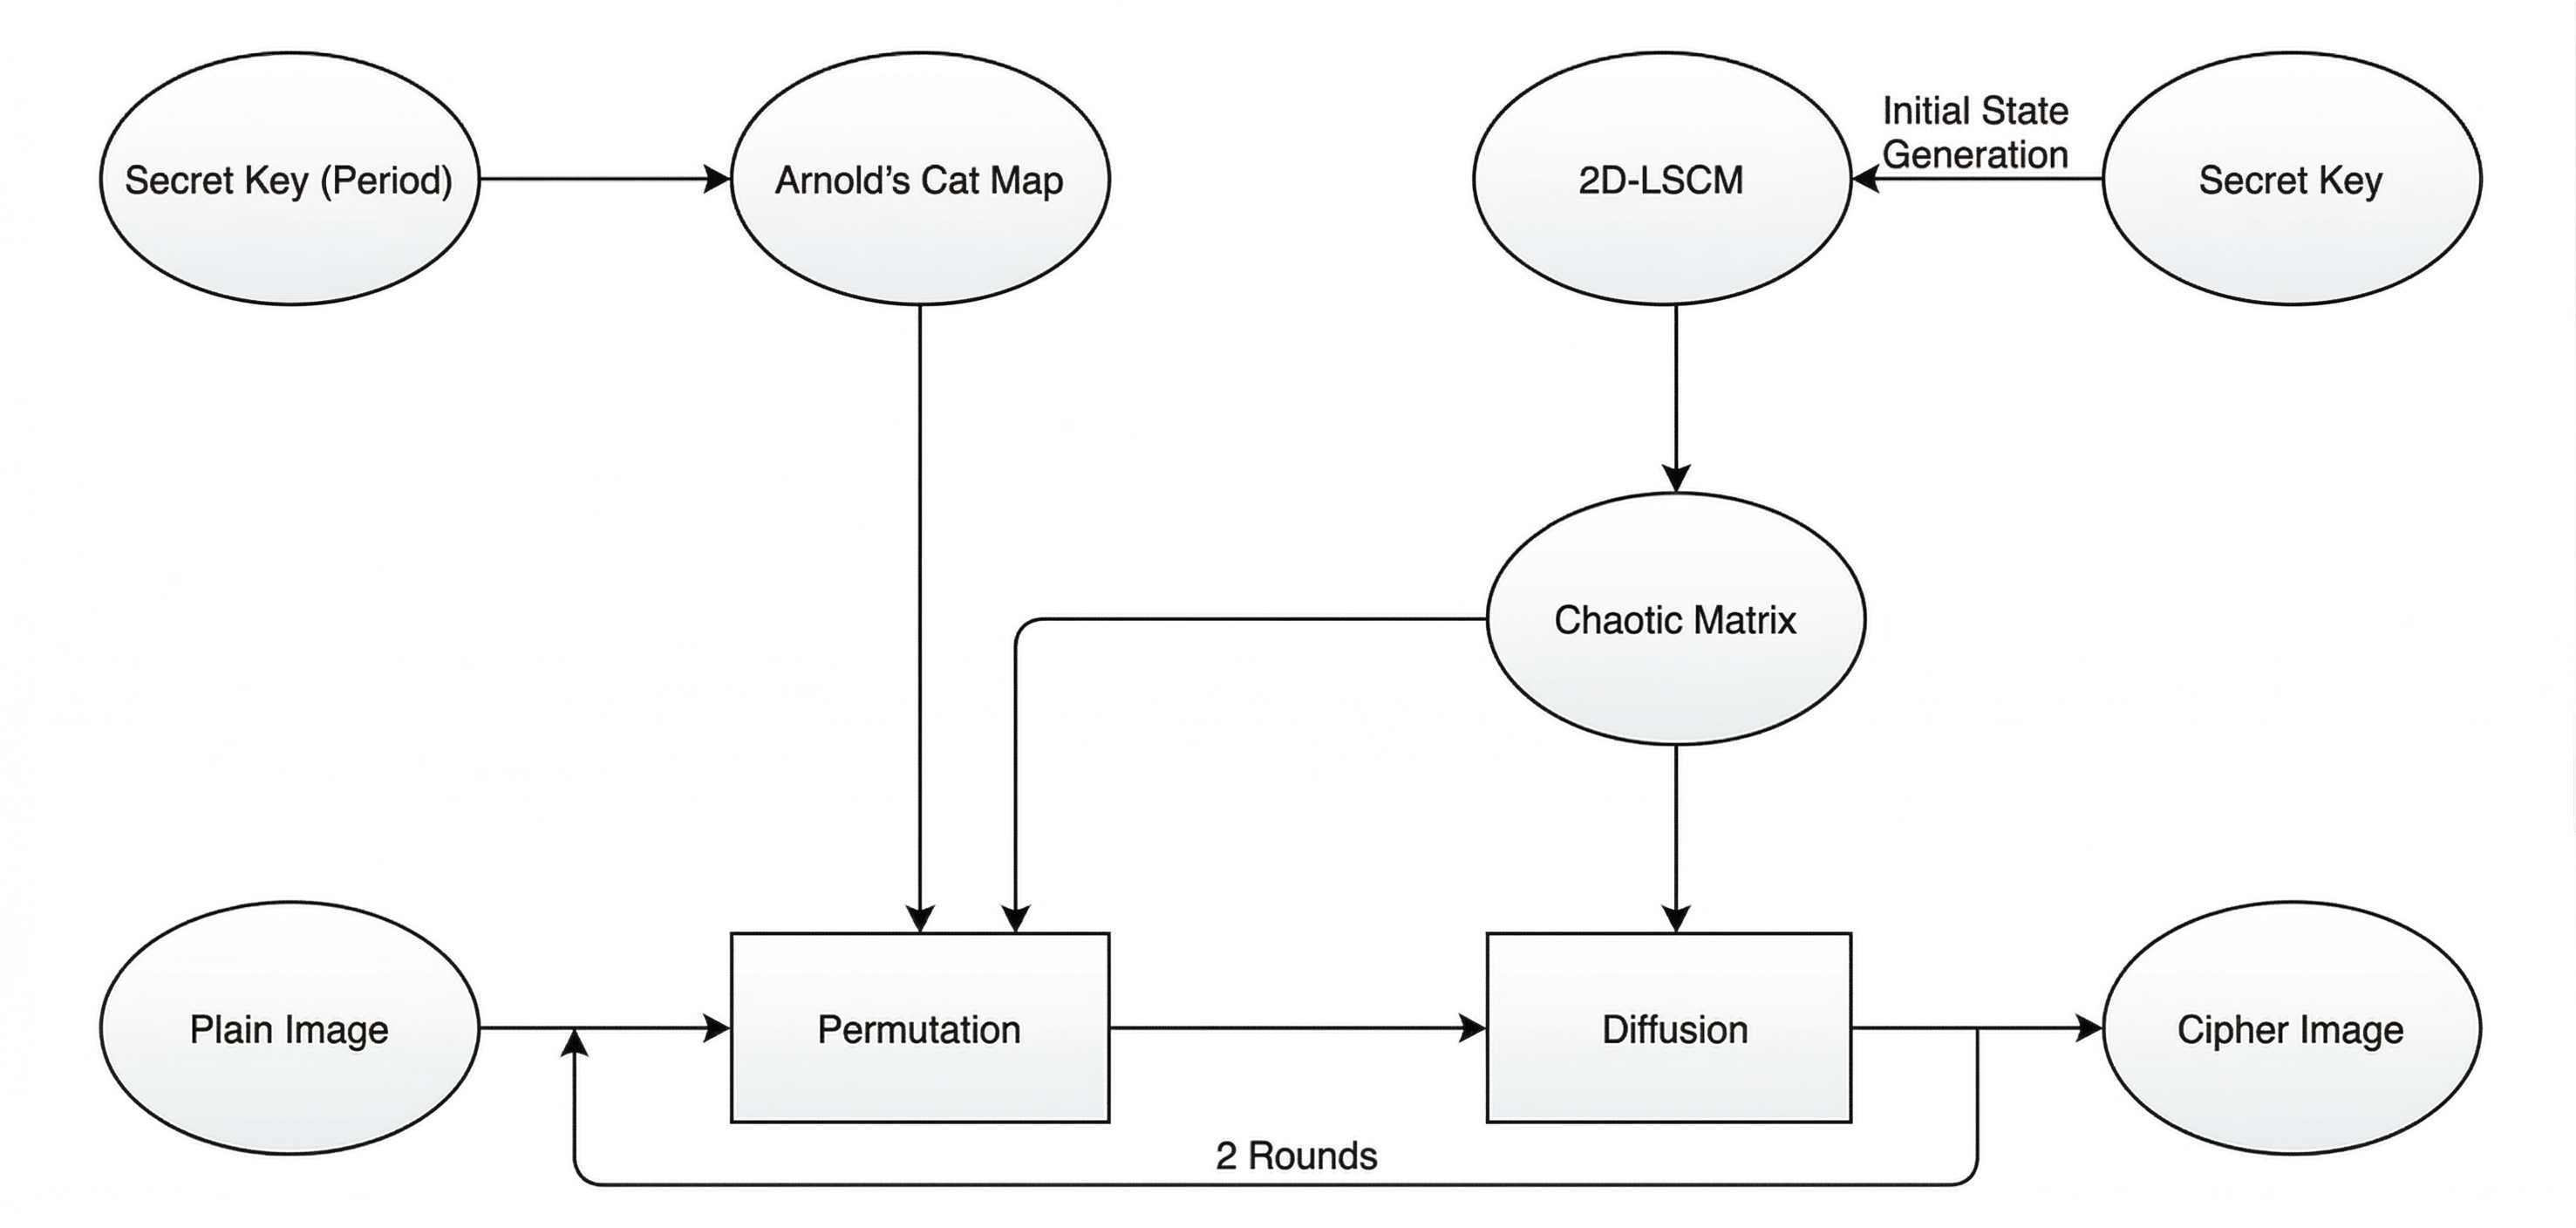
\includegraphics[width=0.9\linewidth]{images/target_methodology.png}
\caption{Encryption process of the target scheme}
\end{figure}

% -----------------------------------------------------------------------
\subsection{Chosen-Plaintext Attack Framework}

The adversary is assumed to have black-box access to an encryption oracle $\mathcal{E}(\cdot)$ that, given any $n \times n$ image $P$, returns the corresponding ciphertext $C = \mathcal{E}(P)$ under an unknown fixed key $(K_1, K_2)$:
\[
C = \mathcal{E}(P).
\]
The adversary has no knowledge of any internal parameters: $x_0$, $y_0$, $\theta$, $P_i$, the chaotic matrix $X$, or the permutation map $\mathcal{M}$.

The exploitable structural weakness is the \emph{plaintext-independence} of all key material. Because the 2D-LSCM sequence $\{x_i\}$ and the derived permutation map $\mathcal{M}$ are functions solely of the secret key—not of the image being encrypted—they remain identical across all images of the same dimensions under the same key. This renders them static equivalent keys, a well-documented vulnerability class in chaos-based cipher design.

The attack proceeds through three phases: (i) keystream extraction by encrypting a zero-valued image, (ii) permutation map reconstruction via structured probe images, and (iii) full decryption of any target ciphertext from the recovered parameters. The data complexity is $n+1$ oracle queries for an $n \times n$ image, and the total computational cost is $\mathcal{O}(n^3)$, dominated by the Arnold map applications in Phase 2.

\begin{figure}[H]
\centering
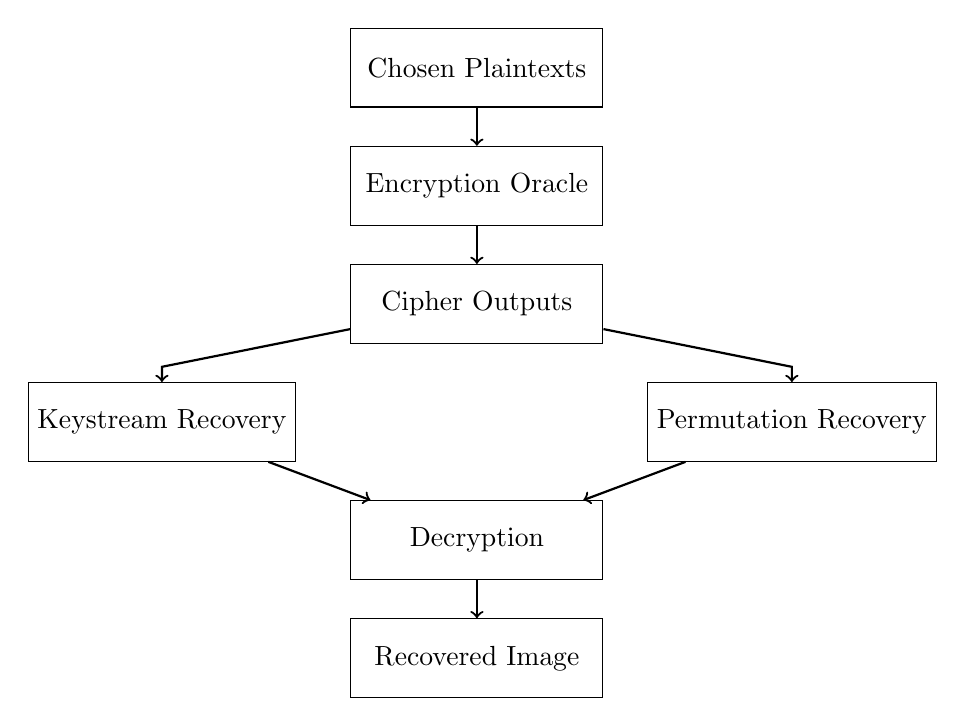
\begin{tikzpicture}[
block/.style={draw, rectangle, minimum width=3.2cm, minimum height=1cm, align=center},
arrow/.style={->, thick}
]
\node[block] (input) at (0,6) {Chosen Plaintexts};
\node[block] (oracle) at (0,4.5) {Encryption Oracle};
\node[block] (cipher) at (0,3) {Cipher Outputs};
\node[block] (ks) at (-4,1.5) {Keystream Recovery};
\node[block] (perm) at (4,1.5) {Permutation Recovery};
\node[block] (decrypt) at (0,0) {Decryption};
\node[block] (out) at (0,-1.5) {Recovered Image};
\draw[arrow] (input) -- (oracle);
\draw[arrow] (oracle) -- (cipher);
\draw[arrow] (cipher) -- (-4,2.2) -- (ks);
\draw[arrow] (cipher) -- (4,2.2) -- (perm);
\draw[arrow] (ks) -- (decrypt);
\draw[arrow] (perm) -- (decrypt);
\draw[arrow] (decrypt) -- (out);
\end{tikzpicture}
\caption{Block diagram of the proposed chosen-plaintext attack showing keystream recovery, permutation recovery, and final decryption without the secret key.}
\label{fig:cpa}
\end{figure}

% -----------------------------------------------------------------------444


\begin{algorithm}[H]
\LinesNumbered
\caption{Chosen-Plaintext Attack on the Target Scheme}
\label{alg:cpa}
\SetAlgoLined
\KwIn{Encryption oracle $\mathcal{E}(\cdot)$; target ciphertext $C$; image size $n$.}
\KwOut{Recovered plaintext $\hat{P}$.}
\BlankLine
\tcp{Phase 1: Keystream Recovery}
$C^{(0)} \leftarrow \mathcal{E}(\mathbf{0}_{n \times n})$ \;
Compute $\hat{X}_i$ for all $i$ using Eq.~\eqref{eq:keystream_recovery}\;
\BlankLine
\tcp{Phase 2: Permutation Map Recovery}
\For{$j = 1$ \KwTo $n$}{
    Construct $P^{(j)}$\;
Set $P^{(j)}_{r,j} \leftarrow r$ for all $r$\;
Set $P^{(j)}_{r,k} \leftarrow 0$ for all $k \neq j$\;

Compute $Q^{(j)} \leftarrow \mathrm{ACM}^{(3n+1-P_i)}\bigl(P^{(j)}\bigr)$\;

$C^{(j)} \leftarrow \mathcal{E}(Q^{(j)})$\;

$\hat{T}^{(j)} \leftarrow \mathcal{D}_{\hat{X}}(C^{(j)})$\;

$\hat{\sigma}_j \leftarrow \hat{T}^{(j)}[:,j]$\;
}
\BlankLine
\tcp{Phase 3: Decryption of Target Ciphertext}
$\hat{T} \leftarrow \mathcal{D}_{\hat{X}}(C)$\;
\For{$j = 1$ \KwTo $n$}{
    $\hat{S}[\hat{\sigma}_j(:),\, j] \leftarrow \hat{T}[:,j]$\;
}
$\hat{P} \leftarrow \mathrm{ACM}^{(3n+1-\tilde{P}_i)}(\hat{S})$\;
\Return $\hat{P}$
\end{algorithm}


\subsection{Phase 1: Keystream Recovery via a Zero Plaintext}

This phase exploits the encryption of an all-zero image to decouple the diffusion layer from the permutation layer and directly expose the keystream.

\subsubsection{Structural Observation}

Let $\mathbf{0}$ denote the $n \times n$ all-zero image and let $C^{(0)} = \mathcal{E}(\mathbf{0})$.

\textbf{Step 1 (Arnold's Cat Map acts as the identity on a zero image).}
Arnold's Cat Map permutes pixel \emph{coordinates} while leaving pixel \emph{values} unchanged. Because every pixel of $\mathbf{0}$ carries the value zero, the map produces the same all-zero image irrespective of the iteration count:
\begin{equation}
\mathrm{ACM}^{P_i}(\mathbf{0}) = \mathbf{0}.
\end{equation}

\textbf{Step 2 (2D-LSCM column permutation acts as the identity on a zero image).}
The column-wise permutation step rearranges rows within column $j$ according to a permutation $\sigma_j$ derived from chaotic matrix $X$. When $P = \mathbf{0}$, every element selected by the permutation equals zero, so:
\begin{equation}
T^{(0)} = \mathbf{0}.
\end{equation}

\textbf{Step 3 (Diffusion collapses to a pure keystream recurrence).}
With $T^{(0)}_i = 0$ for all $i$, the diffusion equation~\eqref{eq:diffusion_enc} simplifies. Substituting and rearranging yields:
\begin{equation}
C^{(0)}_1 = X_1
\end{equation}
\begin{equation}
C^{(0)}_2 = X_1 + X_2 \bmod F
\end{equation}
\begin{equation}
C^{(0)}_i = C^{(0)}_{i-1} + C^{(0)}_{i-2} + X_i \bmod F, \quad i \geq 3.
\end{equation}
Rearranging gives the keystream recovery formula:
\begin{equation}
\boxed{
\hat{X}_i =
\begin{cases}
C^{(0)}_1, & i = 1,\\[4pt]
\bigl(C^{(0)}_2 - C^{(0)}_1\bigr) \bmod F, & i = 2,\\[4pt]
\bigl(C^{(0)}_i - C^{(0)}_{i-1} - C^{(0)}_{i-2}\bigr) \bmod F, & i \geq 3.
\end{cases}
}
\label{eq:keystream_recovery}
\end{equation}

\subsubsection{Correctness of Keystream Recovery}

\begin{proposition}
Every value $\hat{X}_i$ recovered by Eq.~\eqref{eq:keystream_recovery} satisfies $\hat{X}_i = X_i$ for $i = 1, \ldots, N$.
\end{proposition}

\begin{proof}
For $i=1$: directly $\hat{X}_1 = C^{(0)}_1 = X_1$. For $i=2$: $\hat{X}_2 = (C^{(0)}_2 - C^{(0)}_1) \bmod F = X_2$. For $i \geq 3$: by induction, assuming $\hat{X}_k = X_k$ for all $k < i$, we have $\hat{X}_i = (C^{(0)}_i - C^{(0)}_{i-1} - C^{(0)}_{i-2}) \bmod F = X_i$.
\end{proof}

\noindent The complete keystream is thus recovered exactly from a \emph{single} oracle query.

% -----------------------------------------------------------------------
\subsection{Phase 2: Permutation Map Reconstruction}

With the keystream $\{\hat{X}_i\}$ in hand, we reconstruct the full permutation map $\mathcal{M}$ using exactly $n$ additional oracle queries.

\subsubsection{Permutation Structure}

From the encryption process, the permutation stage applies Arnold's Cat Map for $P_i$ iterations and then performs a column-wise sorting step driven by the chaotic matrix $X$. Specifically, for column $j$, if $\sigma_j = \mathrm{argsort}(X[:,j])$ is the permutation induced by sorting that column, the output satisfies
\begin{equation}
T[:,j] = S[\sigma_j, j],
\end{equation}
where $S = \mathrm{ACM}^{P_i}(P)$. The attacker seeks to determine $\mathcal{M}[:,j] = \sigma_j$ for every column.

\subsubsection{Probe Plaintext Design}

For each column index $j \in \{1, \ldots, n\}$, a probe image $P^{(j)}$ is constructed so that column $j$ encodes the row-index sequence $0, 1, \ldots, n-1$ and every other column is identically zero:
\begin{equation}
P^{(j)}_{r,c} =
\begin{cases}
r, & c=j,\\
0, & c \neq j.
\end{cases}
\end{equation}
To neutralize the Arnold preprocessing, the probe submitted to the oracle is the $P_i$-step pre-image of $P^{(j)}$ under the Arnold map, exploiting the map's periodicity:
\begin{equation}
Q^{(j)} = \mathrm{ACM}^{-P_i}\bigl(P^{(j)}\bigr) = \mathrm{ACM}^{(3n+1-P_i)}\bigl(P^{(j)}\bigr).
\end{equation}

\subsubsection{Oracle Output and Permutation Recovery}

When the oracle processes $Q^{(j)}$, the Arnold step undoes the pre-imaging, so that the effective input to the column-sort is precisely $P^{(j)}$. Since column $j$ of $P^{(j)}$ encodes the row indices $r$, the column-sort directly reads out the permutation:
\begin{equation}
T^{(j)}[\ell,j] = \sigma_j(\ell), \qquad \ell = 1, \ldots, n.
\end{equation}
All other columns are zero, so they carry no extraneous information. The oracle then applies diffusion to yield $C^{(j)} = \mathcal{E}(Q^{(j)})$. Inverting the diffusion using the recovered $\hat{X}$:
\begin{equation}
\hat{T}^{(j)}_i =
\begin{cases}
\bigl(C^{(j)}_1 - C^{(j)}_{N} - C^{(j)}_{N-1} - \hat{X}_1\bigr) \bmod F, & i=1,\\[4pt]
\bigl(C^{(j)}_2 - C^{(j)}_1 - C^{(j)}_{N} - \hat{X}_2\bigr) \bmod F, & i=2,\\[4pt]
\bigl(C^{(j)}_i - C^{(j)}_{i-1} - C^{(j)}_{i-2} - \hat{X}_i\bigr) \bmod F, & i \geq 3,
\end{cases}
\label{eq:inv_diff_probe}
\end{equation}
from which the permutation indices for column $j$ are read directly:
\begin{equation}
\hat{\sigma}_j(\ell) = \hat{T}^{(j)}[\ell, j], \qquad \ell = 1, \ldots, n.
\end{equation}
Iterating over all $j = 1, \ldots, n$ completes reconstruction of $\hat{\mathcal{M}}$.

\begin{proposition}
The recovered map satisfies $\hat{\mathcal{M}} = \mathcal{M}$ exactly.
\end{proposition}

\begin{proof}
The probe design guarantees $T^{(j)}[\ell,j] = \sigma_j(\ell)$. Since Proposition~1 guarantees $\hat{X}_i = X_i$ for all $i$, the inverse diffusion in Eq.~\eqref{eq:inv_diff_probe} recovers $\hat{T}^{(j)} = T^{(j)}$ without error, whence $\hat{\sigma}_j = \sigma_j$ for every $j$.
\end{proof}

% -----------------------------------------------------------------------
\subsection{Phase 3: Complete Decryption of Arbitrary Ciphertexts}

Armed with the recovered keystream $\hat{X}$ and permutation map $\hat{\mathcal{M}}$, decryption of any ciphertext $C = \mathcal{E}(P)$ proceeds in three steps without reference to the secret key.

\textbf{Step 1 (Inverse diffusion).}
Compute the permuted image $\hat{T}$ from $C$ via the inverse diffusion operator:
\begin{equation}
\hat{T} = \mathcal{D}_{\hat{X}}(C).
\end{equation}
By Proposition~1, $\hat{T} = T$ exactly.

\textbf{Step 2 (Inverse column permutation).}
For each column $j$, reverse the 2D-LSCM sort using $\hat{\mathcal{M}}$:
\begin{equation}
\hat{S}[\hat{\sigma}_j(\ell),\, j] = \hat{T}[\ell,\, j], \qquad \ell = 1, \ldots, n,
\end{equation}
recovering $\hat{S} = S = \mathrm{ACM}^{P_i}(P)$.

\textbf{Step 3 (Inverse Arnold's Cat Map).}
Apply the Arnold map $(3n+1 - P_i)$ times to $\hat{S}$, exploiting the map's periodicity to compute the inverse via forward iteration:
\begin{equation}
\hat{P} = \mathrm{ACM}^{-P_i}(\hat{S}) = \mathrm{ACM}^{(3n+1-P_i)}(\hat{S}).
\end{equation}
Since $\hat{S} = \mathrm{ACM}^{P_i}(P)$ and Arnold's Cat Map is invertible, $\hat{P} = P$ exactly.

\noindent\textbf{Remark on unknown $P_i$.}
Phase 2 requires knowledge of $P_i$ to construct the probe pre-images $Q^{(j)}$. If $P_i$ is not known, it can be identified by a linear scan: for each candidate $\tilde{P}_i \in \{1, \ldots, 3n\}$, the attacker submits one structured probe and verifies whether column $j$ of the recovered intermediate image matches the expected pattern $\{0,1,\ldots,n-1\}$. The correct value is found in at most $3n - 1$ additional queries, which does not alter the overall polynomial complexity of the attack.

% -----------------------------------------------------------------------
\subsection{Complexity Analysis}

\textbf{Data complexity.}
The entire attack consumes $1 + n$ oracle queries: one zero-image query in Phase 1 and one query per image column in Phase 2. For a $256 \times 256$ image this amounts to 257 queries—negligible from a practical standpoint.

\textbf{Computational complexity.}
Phase 1 inverts the diffusion over all $N = n^2$ pixels in $\mathcal{O}(n^2)$ time. Phase 2 constructs $n$ probe pre-images, each requiring up to $3n$ Arnold map iterations on an $n \times n$ image; since each iteration costs $\mathcal{O}(n^2)$, Phase 2 runs in $\mathcal{O}(n^3)$ in total. Phase 3 requires $\mathcal{O}(n^2)$. The dominant cost is therefore $\mathcal{O}(n^3)$, matching the complexity of the encryption algorithm itself.

\textbf{Memory complexity.}
The attacker need only store the recovered keystream $\hat{X}$ ($n^2$ entries) and the permutation map $\hat{\mathcal{M}}$ ($n^2$ entries), for a total of $\mathcal{O}(n^2)$ space.
